
\section{Signal extraction}\label{sec:WBoson_SignalExtraction}

The signal and background yields are extracted by fitting the \ETslash\ \ distribution in data. The main background sources come from QCD and electroweak processes. The QCD background includes events where a high $p_{T}$ muon is produced from a semi-leptonic decay of quarks (multi-jet background). Most of these muons come from \PQb\ quark decays and light meson (pion and kaon) decays in flight. The dominant electroweak processes are the \DYToMuMu (Drell-Yan) and \WToTauNu as mentioned in \sect{sec:WBoson_SignalExtraction_EWKBackground}. The shape of the signal and background is estimated by using MET templates to describe the signal and the electroweak backgrounds, and a MET functional form derived from data to describe the multi-jet background as explained in \sect{sec:WBoson_SignalExtraction_QCDBackground}.

The simulated samples of \DYToMuMu , \DYToTauTau , \WToMuNu and \WToTauNu are normalized to the total integrated luminosity recorded in data using the NLO cross sections derived from the \POWHEG MC samples scaled by the number of nucleons in the Pb ion. The normalization is done by reweighing all MC events by a global factor defined as $w_{MC} = (\sigma\times\Lumi_{data})/N_{gen}$. In the case of the \ttbar MC, the samples are normalized using $\sigma_{\ttbar} = 45~\nbinv$, which corresponds to the total cross section measured in \pPb collisions at 8.16~\TeV recently published by CMS \cite{HIN-17-002}.

Several corrections are applied to the MC samples before producing the templates, in order to improve the description of the data. First, the event activity in the simulations is reweighed using the energy deposited in the HF calorimeters as explained in \sect{sec:WBoson_Corrections_EventActivityReweighing}. Afterwards, since the muon $\eta_{CM}$ distribution is used to bin the data, the MC muon efficiency is corrected by applying the nominal TnP scale factors event by event, as mentioned in \sect{sec:WBoson_Efficiency_CorrectedEfficiency}. And finally, the resolution of the hadronic recoil component of the MET in MC is corrected as shown in \sect{sec:WBoson_Corrections_RecoilCorrection}, improving the agreement of the MET distribution between data and MC. Once the signal and the EWK MC samples are fully corrected, the MC templates are extracted in each muon $\eta_{CM}$ bin, by creating a histogram of the MET distribution in bins of 2~\GeVc.


\subsection{QCD background}\label{sec:WBoson_SignalExtraction_QCDBackground}


The QCD background is described using a data-driven method. The functional form of the multi-jet \ETslash\ \ distribution is derived by fitting the MET in a region dominated by non-isolated muons selected after inverting the nominal muon isolation cut mentioned in \sect{sec:WBoson_Selection_MuonIdentification}. All analysis cuts are applied except for the muon isolation cut. The general strategy is to first determine the dependence of the QCD functional form with respect to the muon isolation and then extrapolate the QCD shape down to low muon isolation values (signal region).

The nominal QCD \ETslash\ \ functional form is based on a modified version of the Rayleigh distribution as shown in \eq{eq:QCD_Nominal}.

\begin{equation}
f_{QCD}\left(x\right) = x {e}^{-{{x}^{2}}/{\left(2\left(\sigma_{0} + \sigma_{1}\tilde{x} + \sigma_{2}\left(2{\tilde{x}}^{2}-1\right)\right)^{2}\right)}} \quad \textrm{, where} \quad \tilde{x} = (x/50) - 1
\label{eq:QCD_Nominal}
\end{equation}

The free parameters are $\sigma_{0}$ ,  $\sigma_{1}$ and $\sigma_{2}$. The fit parameters have been arranged following a Chebyshev polynomial of second order, to reduce the correlation between parameters and improve the stability of the fits.

In order to derive the muon isolation dependence of the QCD parameters, the \ETslash\ \ distribution function is fitted over the following five muon isolation bins : [ 0.4 , 0.5 , 0.6 , 0.7 , 0.8 , 0.9 ]. The normalization of the QCD background is left free in the fits to the data.

The bins with lower muon isolation values ($\text{iso} < 0.4$) are discarded due to the large contamination from EWK processes. The dependence of the three parameters $\sigma_{0}$ ,  $\sigma_{1}$ and $\sigma_{2}$ with the muon isolation variable is fitted by a linear function. The results of the linear fits are then used to  extrapolate the shape of the QCD background to the signal region (average muon isolation of 0.03), as shown in \fig{fig:QCD_Extrapolation}. The values of the parameters corresponding to this extrapolation are given in \tab{tab:QCD_Extrapolation}.

\begin{table}[htbp]
  \begin{center}
   \begin{tabular}{|c|c|c|}\hline
    Parameter & $QCD \to \mu^{-}$ & $QCD \to \mu^{+}$ \\\hline
    $\sigma_{0}$ & 14.59$\pm$0.18 & 14.72$\pm$0.17 \\\hline
    $\sigma_{1}$ & 6.30$\pm$0.24 & 6.76$\pm$0.23 \\\hline
    $\sigma_{2}$ & 0.49$\pm$0.15 & 0.47$\pm$0.13 \\\hline
   \end{tabular}
  \end{center}
  \caption{QCD shape parameters in the inclusive $\eta_{CM}$ bin, extrapolated to the signal region ($\text{iso} = 0.03$).}
  \label{tab:QCD_Extrapolation}
\end{table}

\begin{figure}[!htbp]
 \begin{center}
  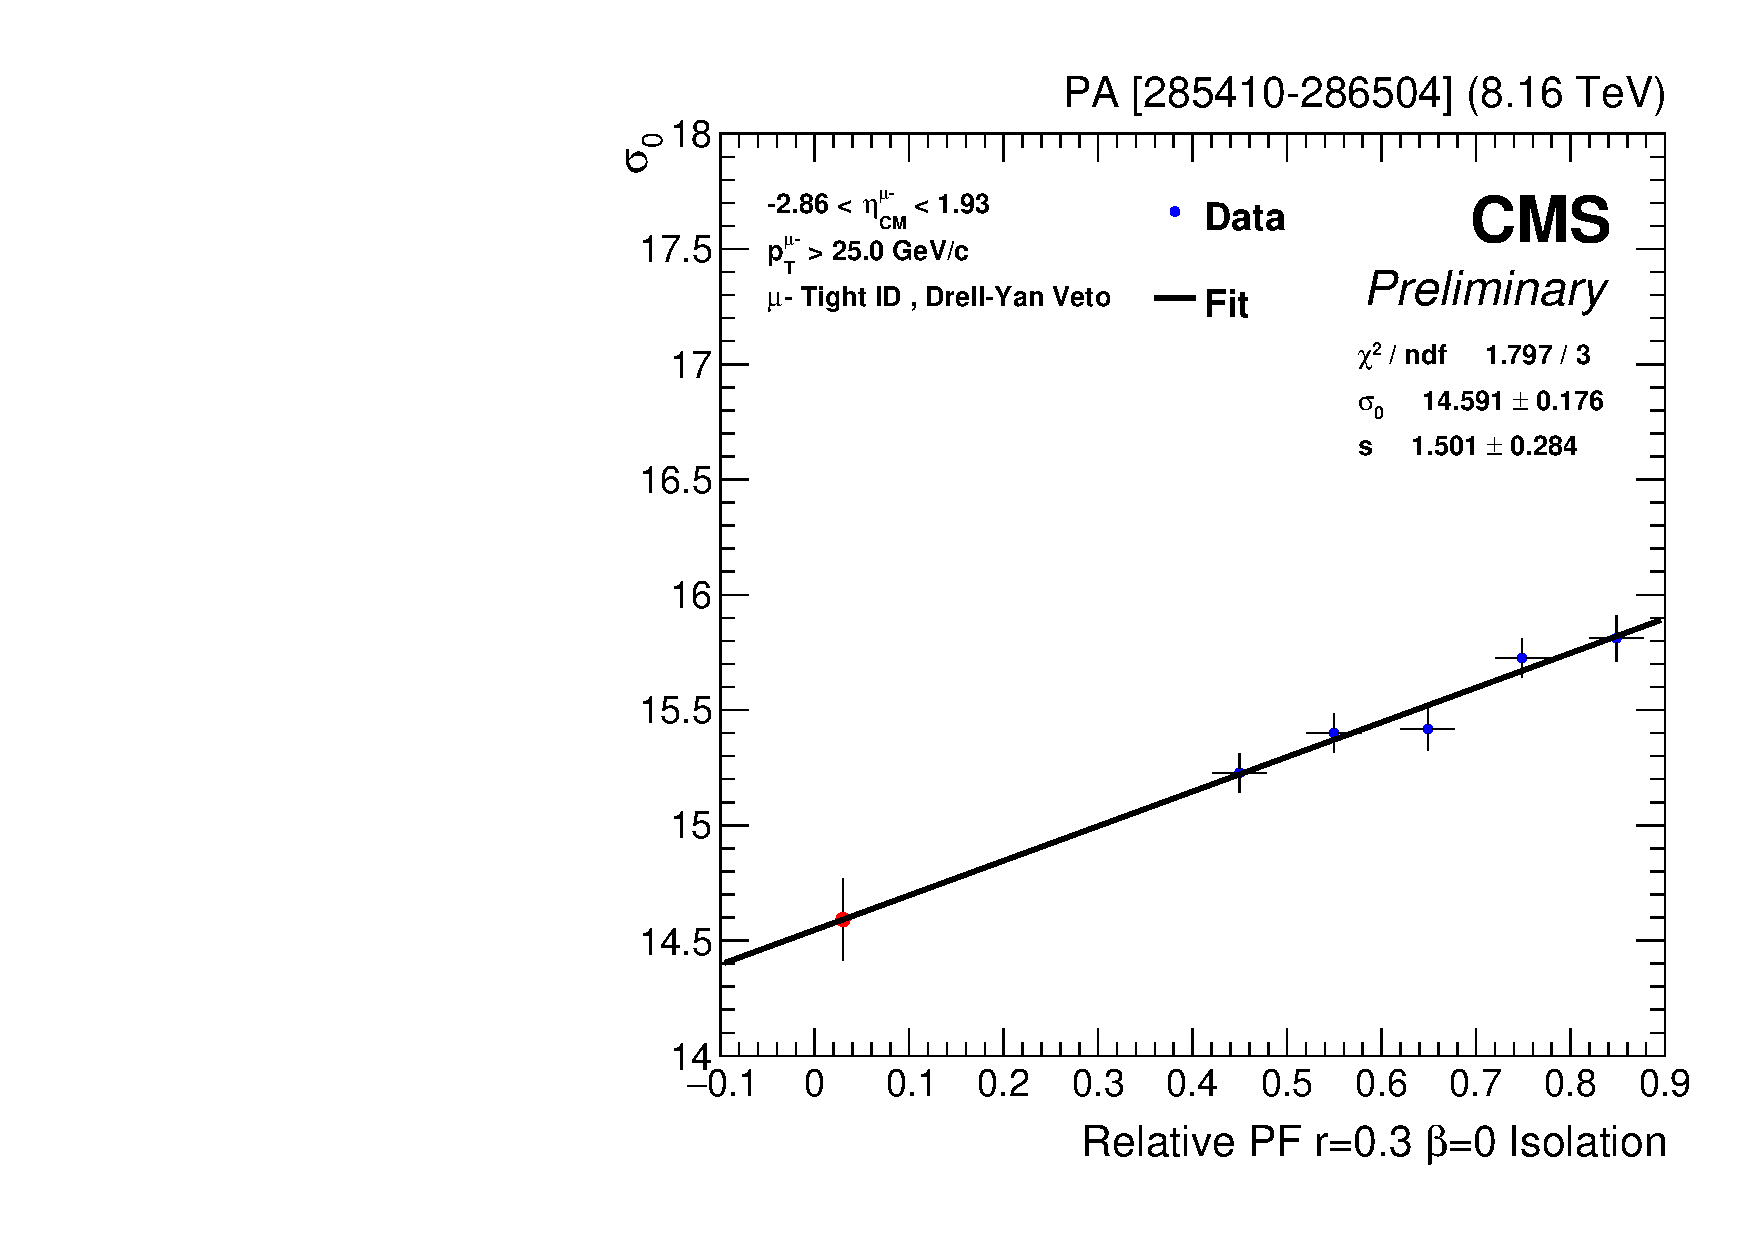
\includegraphics[width=0.27\textwidth]{Figures/WBoson/Analysis/SignalExtraction/QCD_Template/EXTRAPOLATION/PA/graph_Sigma0_QCDToMuMi_PA_-29_eta_19_250_pt_1000000.pdf}
  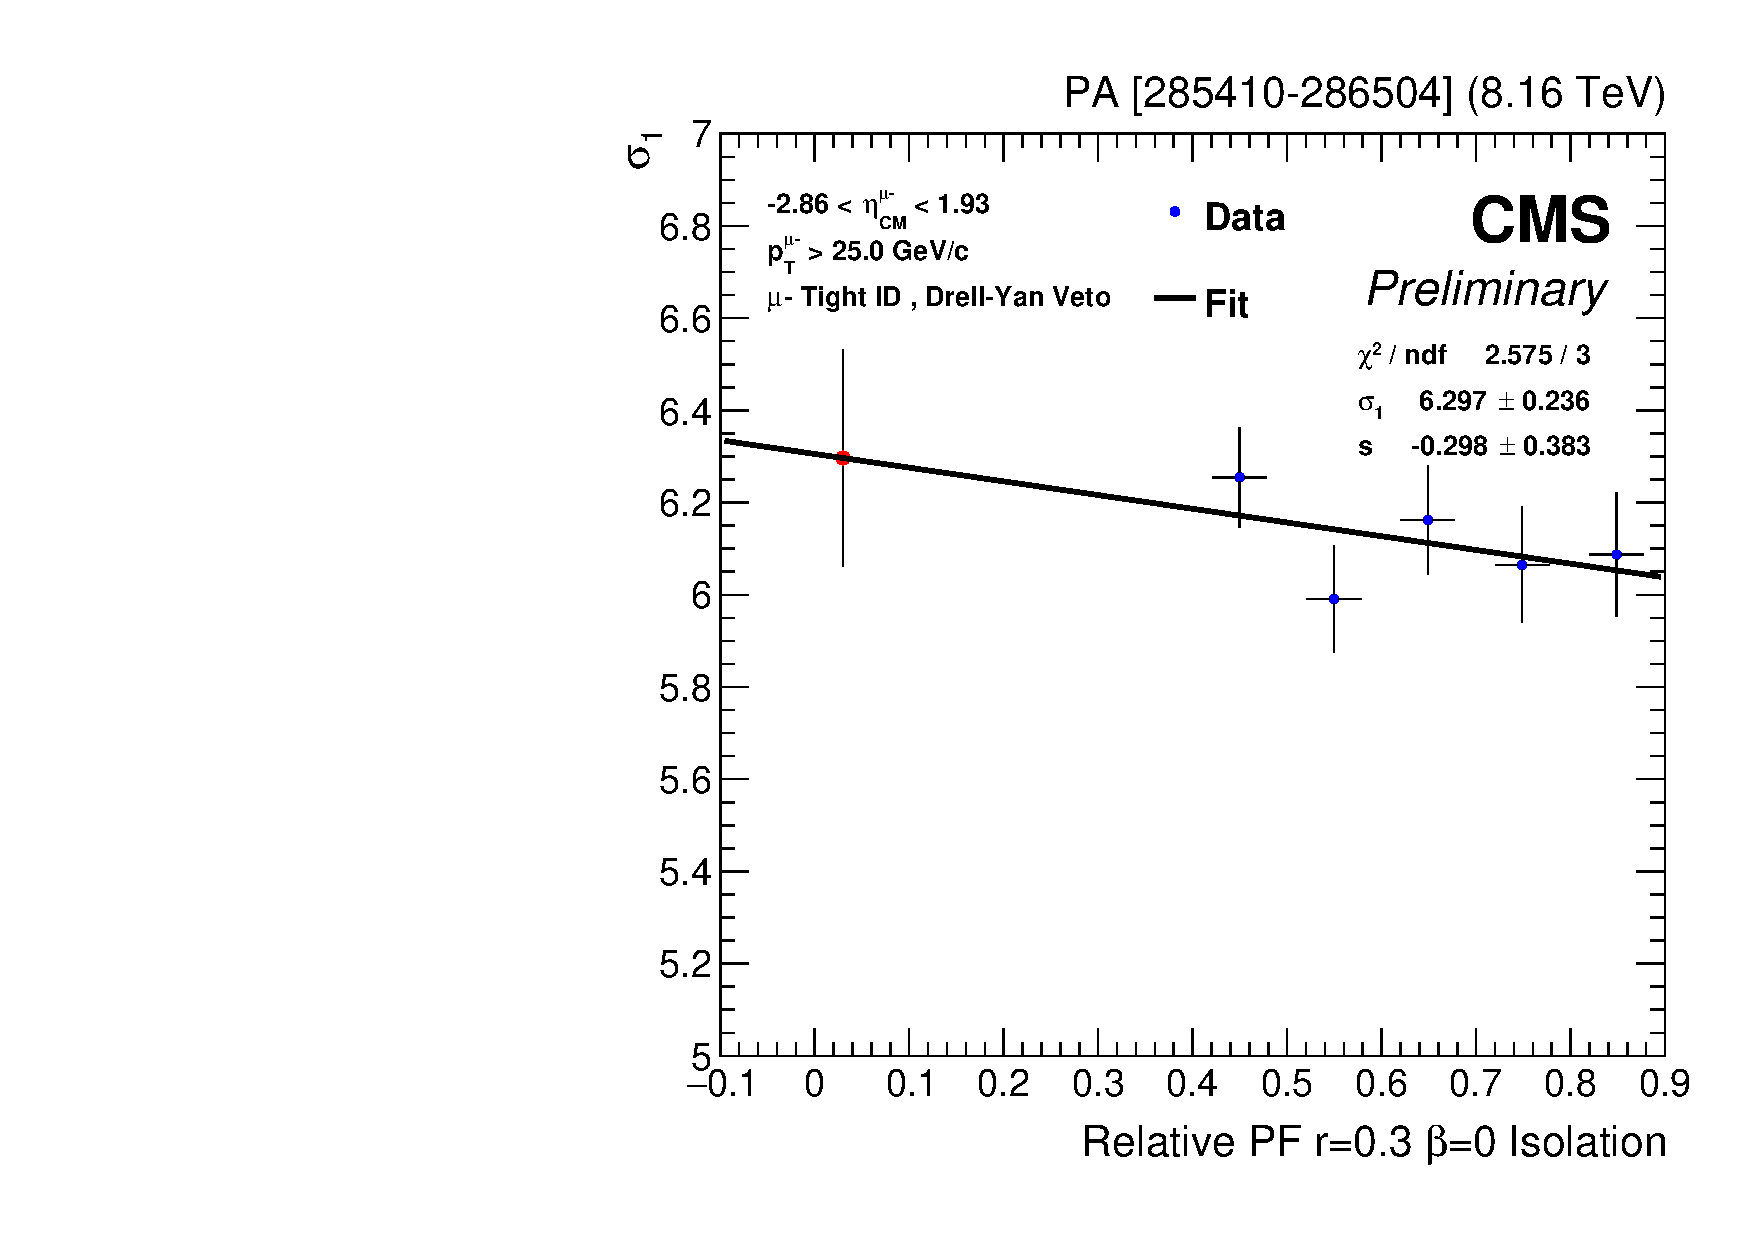
\includegraphics[width=0.27\textwidth]{Figures/WBoson/Analysis/SignalExtraction/QCD_Template/EXTRAPOLATION/PA/graph_Sigma1_QCDToMuMi_PA_-29_eta_19_250_pt_1000000.pdf}
  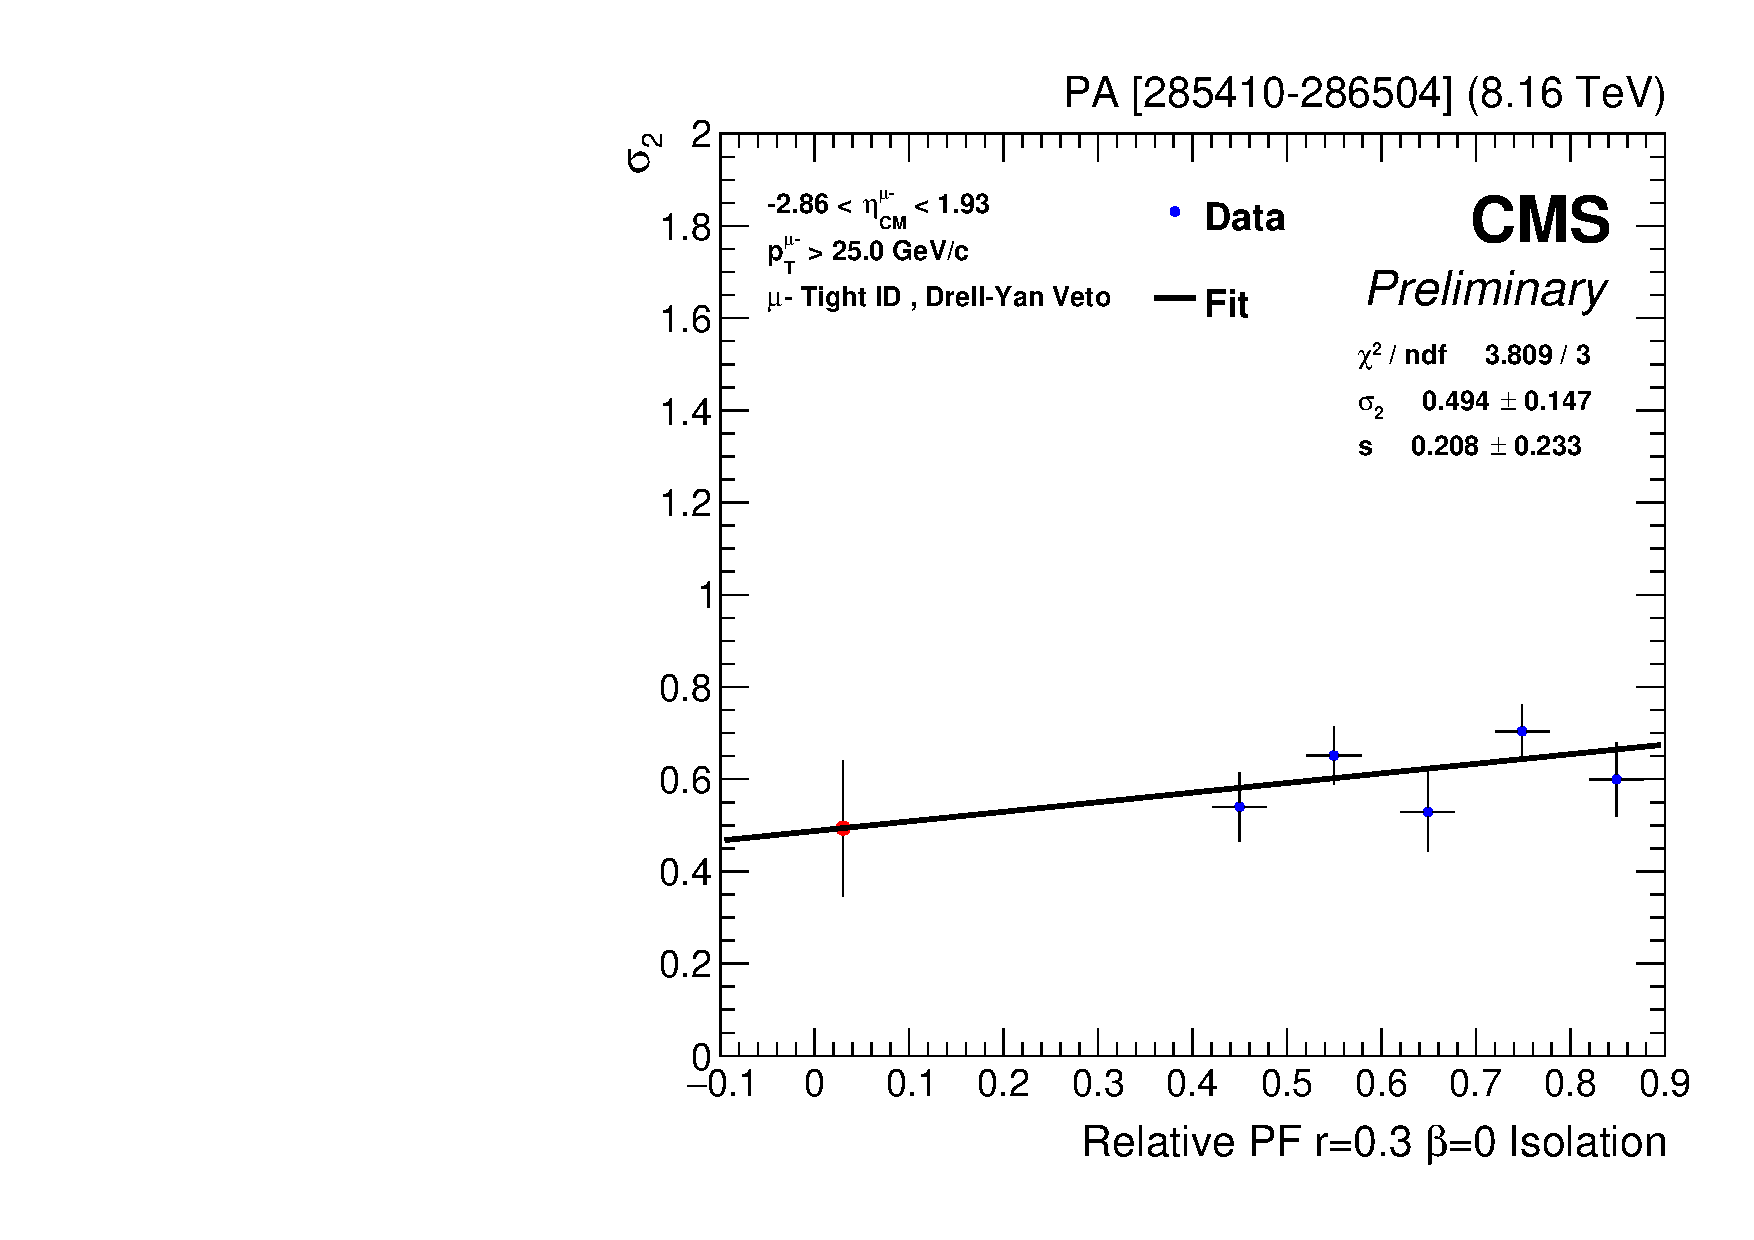
\includegraphics[width=0.27\textwidth]{Figures/WBoson/Analysis/SignalExtraction/QCD_Template/EXTRAPOLATION/PA/graph_Sigma2_QCDToMuMi_PA_-29_eta_19_250_pt_1000000.pdf}
%%
  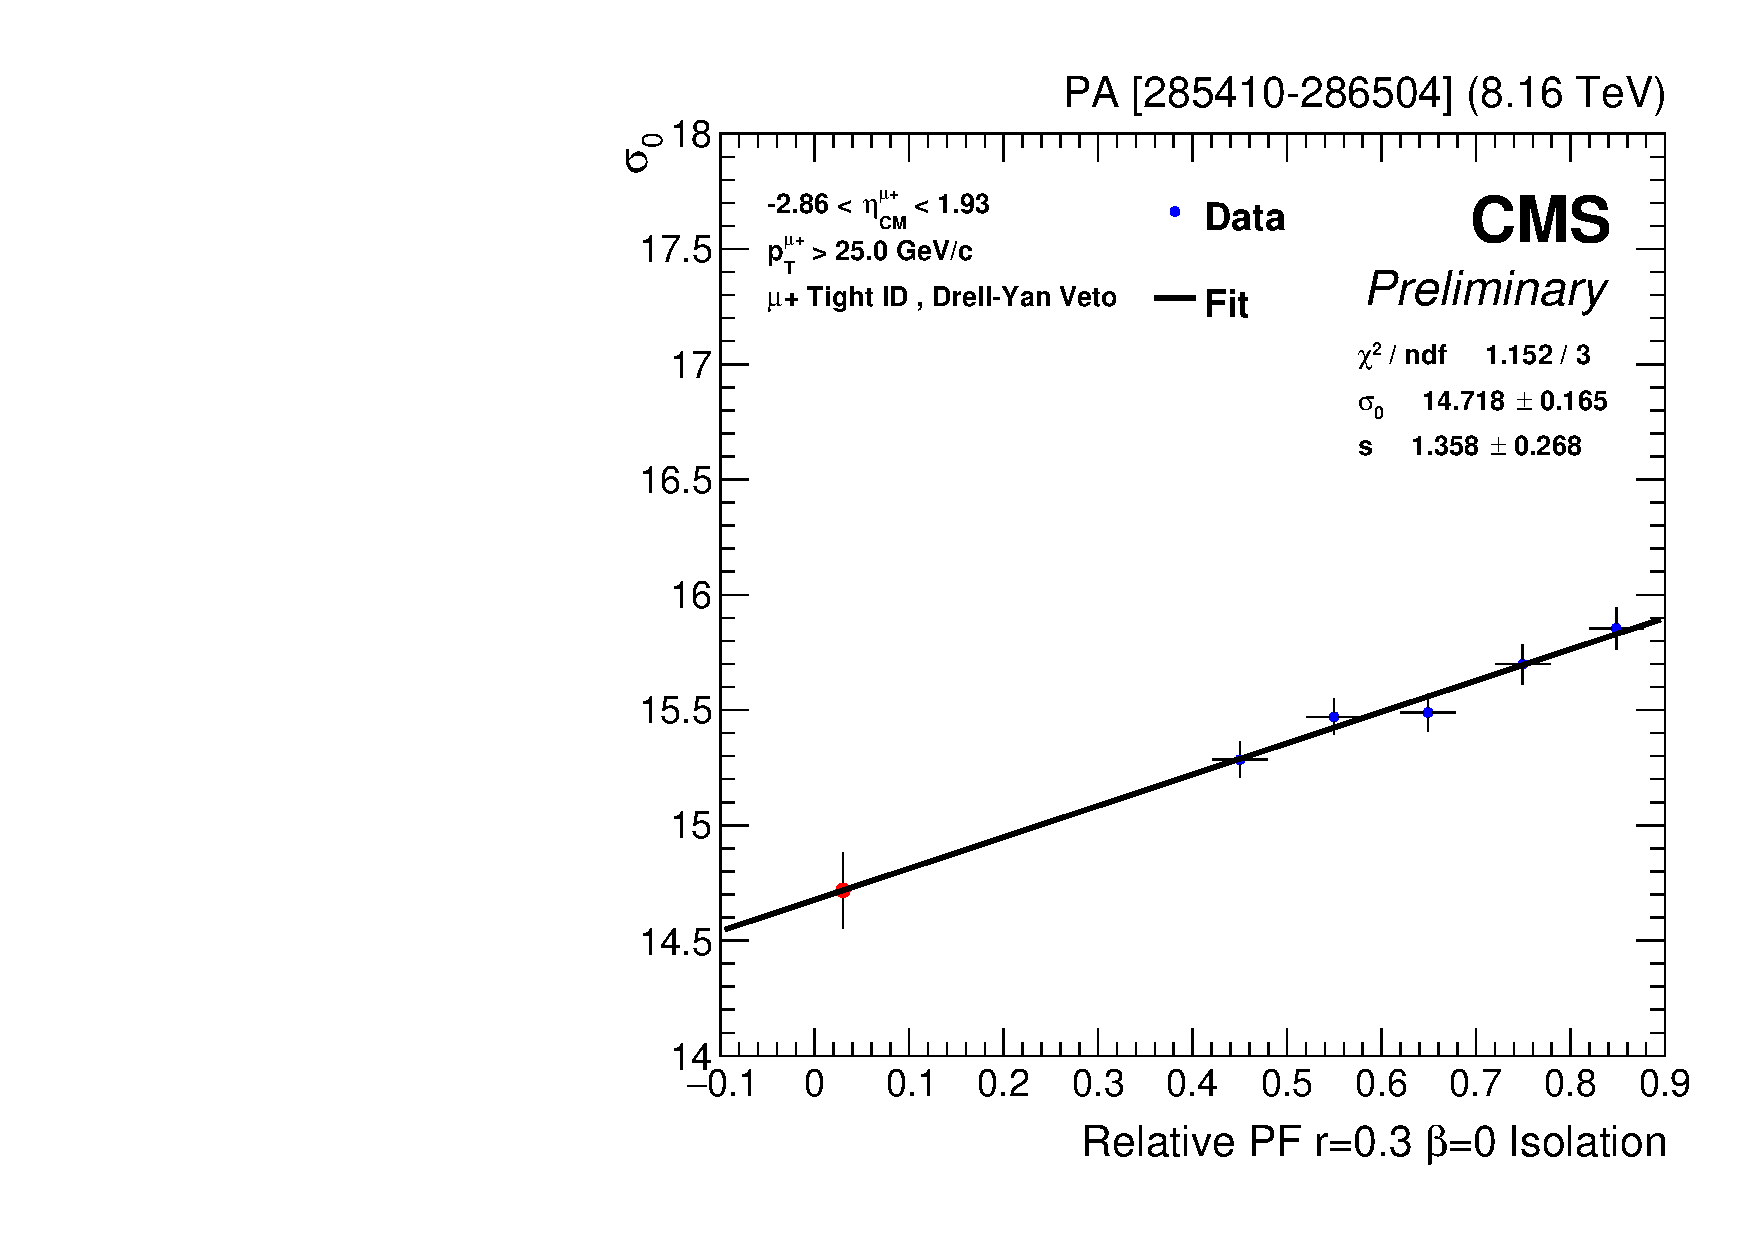
\includegraphics[width=0.27\textwidth]{Figures/WBoson/Analysis/SignalExtraction/QCD_Template/EXTRAPOLATION/PA/graph_Sigma0_QCDToMuPl_PA_-29_eta_19_250_pt_1000000.pdf}
  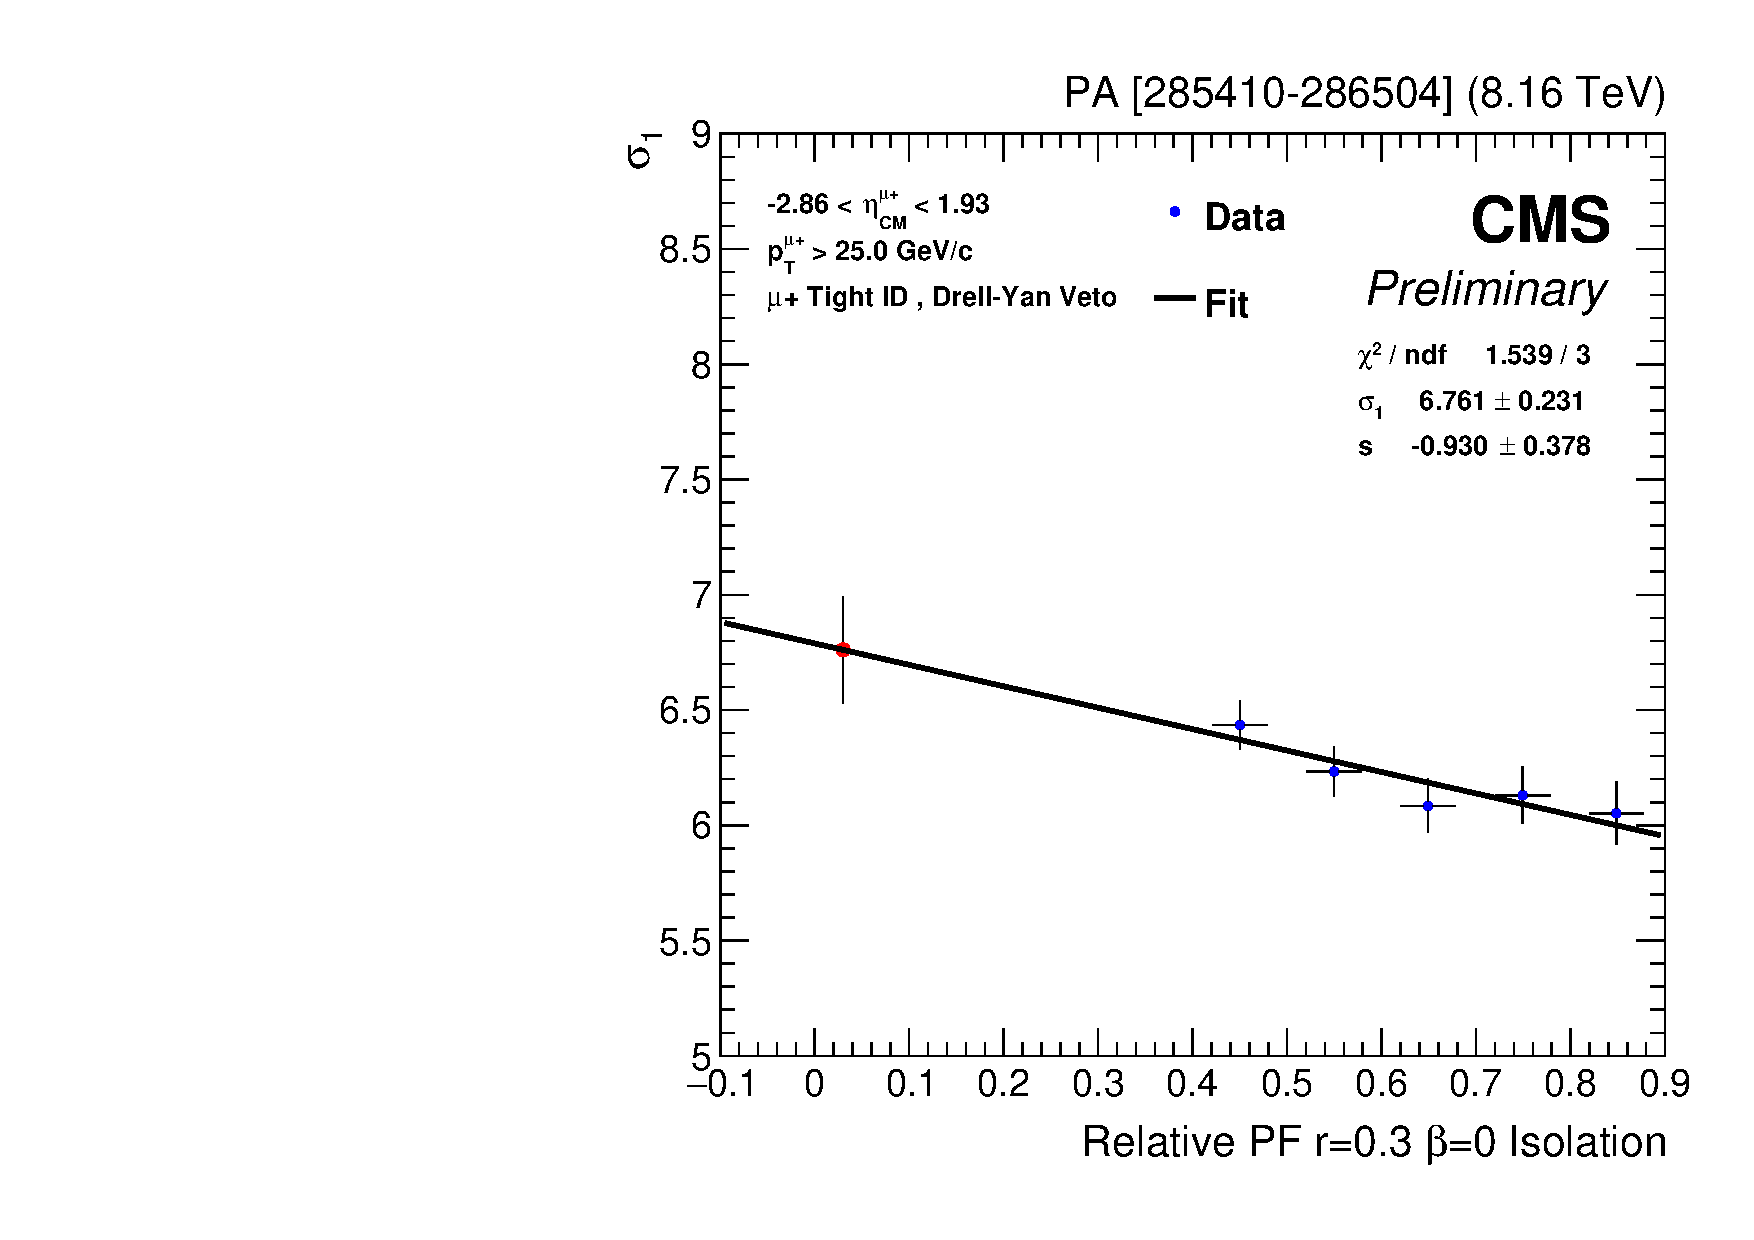
\includegraphics[width=0.27\textwidth]{Figures/WBoson/Analysis/SignalExtraction/QCD_Template/EXTRAPOLATION/PA/graph_Sigma1_QCDToMuPl_PA_-29_eta_19_250_pt_1000000.pdf}
  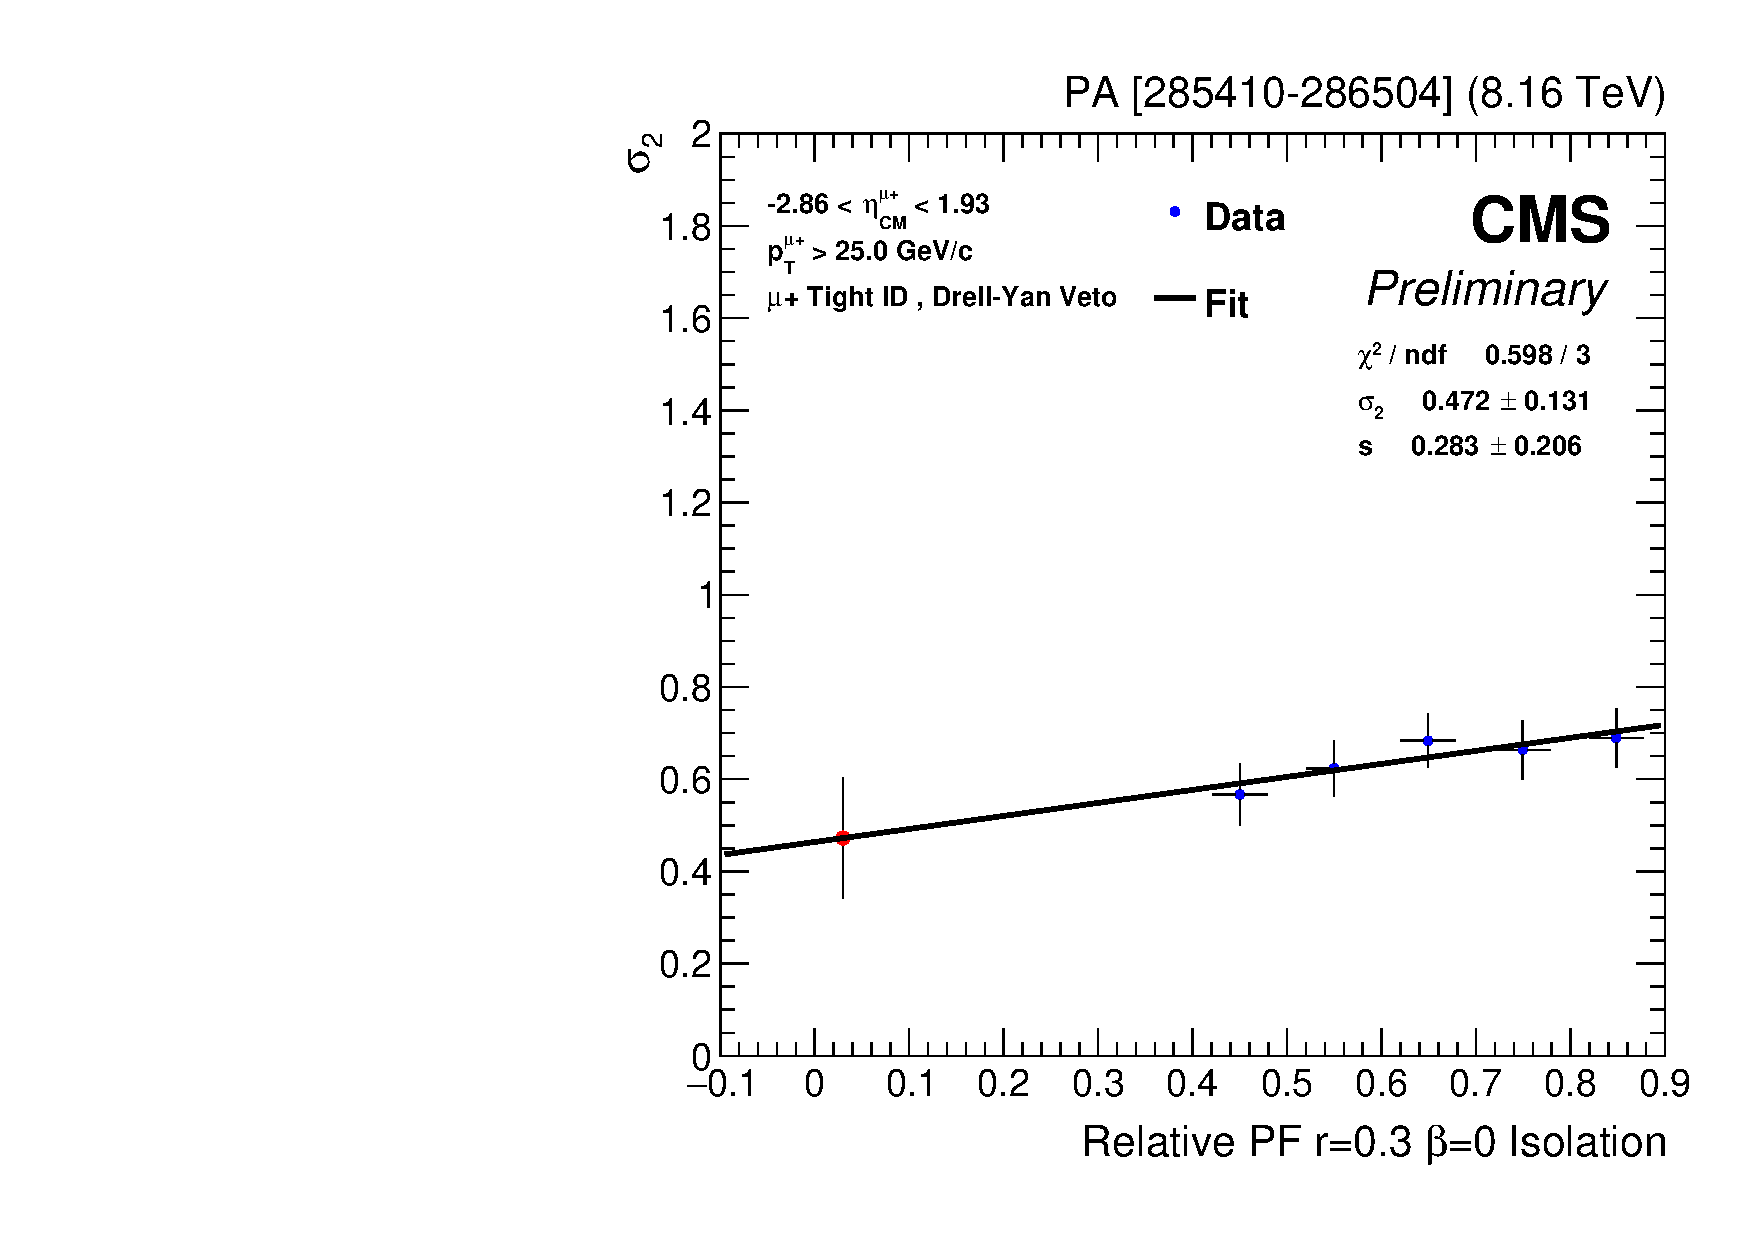
\includegraphics[width=0.27\textwidth]{Figures/WBoson/Analysis/SignalExtraction/QCD_Template/EXTRAPOLATION/PA/graph_Sigma2_QCDToMuPl_PA_-29_eta_19_250_pt_1000000.pdf}
 \end{center}
 \caption{Extrapolation of the parameters of the QCD background shape to the signal region: $\sigma_{0}$ (left), $\sigma_{1}$ (middle) and $\sigma_{2}$ (right), separated in negative (top) and positive (bottom) muon decays. Only the results inclusive in muon $\eta_{CM}$ are shown.}
 \label{fig:QCD_Extrapolation}
\end{figure}

The dependence on $\eta_{CM}$ of the QCD shape has been studied. The extrapolated results do not vary significantly with respect to $\eta_{CM}$ and have been found to be consistent with the $\eta$-inclusive results, within the fit uncertainties. Therefore, the $\eta$-inclusive extrapolated results for each muon charge are used to fix the QCD background shape when fitting the signal.


\subsection{Electroweak background}\label{sec:WBoson_SignalExtraction_EWKBackground}

Among all the electroweak background sources, the dominant one in the \W signal region is the Drell-Yan process. The Drell-Yan background is mainly made of \ZToMuMu events, where one of the muons is produced outside of the detector coverage ($|\eta|<$ 2.4) or did not pass the selection criteria. The other type of EWK sources considered in this analysis are \DYToTauTau, \WToTauNu and \ttbar. The EWK background represents around $13.3\%$ of the events in the signal region, divided as: \DYToMuMu ($9.4\%$), \WToTauNu ($2.4\%$), \DYToTauTau ($1.0\%$) and \ttbar ($0.5\%$). Other EWK processes such as double boson decays have been checked to contribute less than $0.03\%$, so they are not considered.

The contribution of each EWK background is described using \ETslash\ \ templates derived from the MC samples. The MET templates are produced following the procedure explained at the beginning of this section.


\subsection{Fit model}\label{sec:WBoson_SignalExtraction_FitModel}

The raw \WToMuNu yields are extracted by performing an unbinned log-likelihood fit of the observed \ETslash\ \ distribution in each muon $\eta_{CM}$ bin. The fits are done using a combination of binned templates and a continous functional form. The data analysis framework RooFit v3.60 \cite{RooFit} is used to make the fits.

The total fit model includes five contributions: the signal \WToMuNu template ($\mathcal{T}_{W}$), the EWK backgrounds \DYToMuMu, \WToTauNu, \DYToTauTau and \ttbar templates ($\mathcal{T}_{EWK}$), and the QCD data-driven functional form ($\mathcal{F}_{QCD}$). The model used to fit the data is shown in \eq{eq:FitModel}.

\begin{equation}
\resizebox{0.935\textwidth}{!}{%
${ N_{\W} \times \left( {\mathcal{T}_{\W}} + {r_{\DYToMuMu} \cdot \mathcal{T}_{\DYToMuMu}} + {r_{\WToTauNu} \cdot \mathcal{T}_{\WToTauNu}} + {r_{\DYToTauTau} \cdot \mathcal{T}_{\DYToTauTau}} + {r_{\ttbar} \cdot \mathcal{T}_{\ttbar}} \right) } + { N_{QCD} \times \mathcal{F}_{QCD} }$%
}
\label{eq:FitModel}
\end{equation}

The signal and the EWK background shapes are defined based on \ETslash\ \ templates, evaluated from MC simulations. Since the fits become too unstable if the EWK background yields are left free, the following criteria is used to constrain their yields. First, the \DYToMuMu , \WToTauNu, \DYToTauTau and the \ttbar raw yields are expressed in terms of $N_{EWK} = r_{EWK}\times N_{W}$. Afterwards, the ratio of raw yields ($r_{EWK}$) is fixed to its corresponding value derived from MC after having normalized all the MC samples to the recorded integrated luminosity and applied all analysis corrections and selection cuts. This criteria assume that the nuclear modification of the electroweak sources scales in the same way as the \W signal, which is expected at least for the \WToTauNu and the \DY processes.

The QCD contribution, as explained in section~\ref{sec:WBoson_SignalExtraction_QCDBackground}, is taken into account by means of a functional form depending on three parameters. For the fit of the \ETslash\ \  distribution the $\sigma_{0}$ , $\sigma_{1}$ and $\sigma_{2}$ are fixed to the extrapolated values mentioned in \tab{tab:QCD_Extrapolation}.

The \ETslash\ \ distribution is fitted separately for \WToMuNuPl and \WToMuNuMi candidates. Only the signal raw yield ($N_{\W}$) and the QCD normalization ($N_{QCD}$) are left free when fitting the \W signal region. The fits are done in both the inclusive selected events and in bins of muon pseudorapidity in the center of mass frame $\eta_{CM}$.


\subsection{Raw yields}\label{sec:WBoson_SignalExtraction_RawYields}


The results of the fits to the data in each of the different muon $\eta_{CM}$ bins are summarized in \tab{tab:RawYields_WToMuMi_PA} for $\W^{-}$ and in \tab{tab:RawYields_WToMuPl_PA} for $\W^{+}$.

\begin{table}[h!]
  \centering
  \resizebox{\textwidth}{!}{
  \renewcommand{\arraystretch}{1.5}
  \begin{tabular}{|c|*9c|}
    \hline
    $\eta_{CM}$ Range & Total & Fitted & Signal & \DYToMuMu & \WToTauNu & \DYToTauTau & \ttbar & QCD & p-value ($\chi^{2}$)\\
    \hline\hline
    -2.86 , -2.60 & 5210 & 5210 & $4056 \pm 66$ & $563 \pm 9$ & $137 \pm 2$ & $46 \pm 1$ & $3 \pm 0$ & $405 \pm 40$ & 0.42\\
    \hline
    -2.60 , -2.40 & 4308 & 4308 & $3407 \pm 60$ & $465 \pm 8$ & $104 \pm 2$ & $37 \pm 1$ & $4 \pm 0$ & $292 \pm 36$ & 0.31\\
    \hline
    -2.40 , -2.20 & 4273 & 4273 & $3290 \pm 60$ & $450 \pm 8$ & $103 \pm 2$ & $37 \pm 1$ & $5 \pm 0$ & $388 \pm 38$ & 0.26\\
    \hline
    -2.20 , -1.93 & 6423 & 6423 & $4936 \pm 74$ & $659 \pm 10$ & $158 \pm 2$ & $63 \pm 1$ & $12 \pm 0$ & $595 \pm 48$ & 0.53\\
    \hline
    -1.93 , -1.80 & 3140 & 3140 & $2430 \pm 52$ & $309 \pm 7$ & $80 \pm 2$ & $29 \pm 1$ & $8 \pm 0$ & $285 \pm 34$ & 0.51\\
    \hline
    -1.80 , -1.60 & 4822 & 4822 & $3682 \pm 64$ & $438 \pm 8$ & $119 \pm 2$ & $46 \pm 1$ & $19 \pm 0$ & $518 \pm 43$ & 0.46\\
    \hline
    -1.60 , -1.40 & 4727 & 4727 & $3644 \pm 64$ & $395 \pm 7$ & $119 \pm 2$ & $39 \pm 1$ & $18 \pm 0$ & $512 \pm 43$ & 0.85\\
    \hline
    -1.40 , -1.20 & 4521 & 4521 & $3600 \pm 64$ & $347 \pm 6$ & $111 \pm 2$ & $46 \pm 1$ & $21 \pm 0$ & $397 \pm 40$ & 0.03\\
    \hline
    -1.20 , -1.00 & 4626 & 4626 & $3672 \pm 65$ & $312 \pm 6$ & $120 \pm 2$ & $51 \pm 1$ & $23 \pm 0$ & $448 \pm 42$ & 0.57\\
    \hline
    -1.00 , -0.80 & 4722 & 4722 & $3769 \pm 66$ & $284 \pm 5$ & $121 \pm 2$ & $46 \pm 1$ & $31 \pm 1$ & $470 \pm 43$ & 0.87\\
    \hline
    -0.80 , -0.60 & 4198 & 4198 & $3434 \pm 63$ & $247 \pm 5$ & $105 \pm 2$ & $46 \pm 1$ & $29 \pm 1$ & $337 \pm 39$ & 0.82\\
    \hline
    -0.60 , -0.40 & 4648 & 4648 & $3743 \pm 66$ & $253 \pm 4$ & $122 \pm 2$ & $55 \pm 1$ & $37 \pm 1$ & $438 \pm 43$ & 0.09\\
    \hline
    -0.40 , -0.20 & 4344 & 4344 & $3484 \pm 64$ & $233 \pm 4$ & $112 \pm 2$ & $51 \pm 1$ & $34 \pm 1$ & $430 \pm 41$ & 0.16\\
    \hline
    -0.20 , +0.00 & 4474 & 4474 & $3522 \pm 65$ & $267 \pm 5$ & $114 \pm 2$ & $44 \pm 1$ & $37 \pm 1$ & $490 \pm 43$ & 0.01\\
    \hline
    +0.00 , +0.20 & 4643 & 4643 & $3661 \pm 65$ & $318 \pm 6$ & $116 \pm 2$ & $48 \pm 1$ & $39 \pm 1$ & $461 \pm 43$ & 0.00\\
    \hline
    +0.20 , +0.40 & 4638 & 4638 & $3538 \pm 64$ & $343 \pm 6$ & $112 \pm 2$ & $52 \pm 1$ & $43 \pm 1$ & $549 \pm 44$ & 0.00\\
    \hline
    +0.40 , +0.60 & 4718 & 4718 & $3538 \pm 63$ & $396 \pm 7$ & $117 \pm 2$ & $47 \pm 1$ & $38 \pm 1$ & $583 \pm 44$ & 0.30\\
    \hline
    +0.60 , +0.80 & 4552 & 4552 & $3382 \pm 62$ & $456 \pm 8$ & $106 \pm 2$ & $49 \pm 1$ & $34 \pm 1$ & $525 \pm 43$ & 0.64\\
    \hline
    +0.80 , +1.00 & 4637 & 4637 & $3331 \pm 61$ & $496 \pm 9$ & $106 \pm 2$ & $43 \pm 1$ & $39 \pm 1$ & $622 \pm 44$ & 0.00\\
    \hline
    +1.00 , +1.20 & 4612 & 4612 & $3281 \pm 60$ & $545 \pm 10$ & $108 \pm 2$ & $45 \pm 1$ & $27 \pm 0$ & $605 \pm 44$ & 0.54\\
    \hline
    +1.20 , +1.40 & 4053 & 4053 & $2761 \pm 54$ & $532 \pm 11$ & $78 \pm 2$ & $39 \pm 1$ & $22 \pm 0$ & $621 \pm 42$ & 0.11\\
    \hline
    +1.40 , +1.60 & 4251 & 4251 & $2924 \pm 56$ & $625 \pm 12$ & $100 \pm 2$ & $39 \pm 1$ & $21 \pm 0$ & $541 \pm 43$ & 0.16\\
    \hline
    +1.60 , +1.80 & 3844 & 3844 & $2511 \pm 51$ & $620 \pm 13$ & $79 \pm 2$ & $35 \pm 1$ & $15 \pm 0$ & $584 \pm 41$ & 0.06\\
    \hline
    +1.80 , +1.93 & 2640 & 2640 & $1724 \pm 42$ & $443 \pm 11$ & $55 \pm 1$ & $22 \pm 1$ & $9 \pm 0$ & $387 \pm 34$ & 0.44\\
    \hline
  \end{tabular}
  }
  \caption{Raw yields of \WToMuNuMi and background processes, extracted from the nominal fits for each muon $\eta_{CM}$ bin in the combined \pPb and \Pbp collision system. All analysis cuts are applied including the muon $p_{T} > 25$~GeV/c cut. All uncertainties shown are statistical only.}
  \label{tab:RawYields_WToMuMi_PA}
\end{table}


\begin{table}[h!]
  \centering
  \resizebox{\textwidth}{!}{
  \renewcommand{\arraystretch}{1.5}
  \begin{tabular}{|c|*9c|}
    \hline
    $\eta_{CM}$ Range & Total & Fitted & Signal & \DYToMuMu & \WToTauNu & \DYToTauTau & \ttbar & QCD & p-value ($\chi^{2}$)\\
    \hline\hline
    -2.86 , -2.60 & 4465 & 4465 & $3361 \pm 59$ & $589 \pm 10$ & $68 \pm 1$ & $46 \pm 1$ & $3 \pm 0$ & $397 \pm 38$ & 0.05\\
    \hline
    -2.60 , -2.40 & 4234 & 4234 & $3253 \pm 58$ & $533 \pm 10$ & $66 \pm 1$ & $37 \pm 1$ & $4 \pm 0$ & $341 \pm 36$ & 0.04\\
    \hline
    -2.40 , -2.20 & 4377 & 4377 & $3350 \pm 60$ & $503 \pm 9$ & $61 \pm 1$ & $37 \pm 1$ & $11 \pm 0$ & $415 \pm 38$ & 0.96\\
    \hline
    -2.20 , -1.93 & 6847 & 6846 & $5266 \pm 76$ & $723 \pm 10$ & $103 \pm 1$ & $55 \pm 1$ & $14 \pm 0$ & $686 \pm 49$ & 0.41\\
    \hline
    -1.93 , -1.80 & 3592 & 3591 & $2769 \pm 56$ & $340 \pm 7$ & $56 \pm 1$ & $30 \pm 1$ & $8 \pm 0$ & $388 \pm 36$ & 0.55\\
    \hline
    -1.80 , -1.60 & 5421 & 5417 & $4311 \pm 70$ & $496 \pm 8$ & $95 \pm 2$ & $51 \pm 1$ & $15 \pm 0$ & $449 \pm 44$ & 0.48\\
    \hline
    -1.60 , -1.40 & 5343 & 5343 & $4382 \pm 70$ & $451 \pm 7$ & $97 \pm 2$ & $46 \pm 1$ & $17 \pm 0$ & $350 \pm 42$ & 0.90\\
    \hline
    -1.40 , -1.20 & 5129 & 5125 & $4198 \pm 70$ & $386 \pm 6$ & $100 \pm 2$ & $42 \pm 1$ & $22 \pm 0$ & $377 \pm 43$ & 0.12\\
    \hline
    -1.20 , -1.00 & 5382 & 5380 & $4475 \pm 72$ & $344 \pm 6$ & $102 \pm 2$ & $56 \pm 1$ & $26 \pm 0$ & $378 \pm 43$ & 0.23\\
    \hline
    -1.00 , -0.80 & 5467 & 5464 & $4499 \pm 73$ & $314 \pm 5$ & $101 \pm 2$ & $51 \pm 1$ & $30 \pm 0$ & $469 \pm 45$ & 0.05\\
    \hline
    -0.80 , -0.60 & 4738 & 4737 & $3971 \pm 69$ & $251 \pm 4$ & $91 \pm 2$ & $43 \pm 1$ & $28 \pm 0$ & $352 \pm 41$ & 0.18\\
    \hline
    -0.60 , -0.40 & 5349 & 5349 & $4446 \pm 73$ & $263 \pm 4$ & $101 \pm 2$ & $49 \pm 1$ & $36 \pm 1$ & $454 \pm 45$ & 0.16\\
    \hline
    -0.40 , -0.20 & 5027 & 5023 & $4154 \pm 70$ & $246 \pm 4$ & $91 \pm 2$ & $47 \pm 1$ & $35 \pm 1$ & $450 \pm 44$ & 0.12\\
    \hline
    -0.20 , +0.00 & 5161 & 5160 & $4279 \pm 71$ & $276 \pm 5$ & $101 \pm 2$ & $47 \pm 1$ & $38 \pm 1$ & $419 \pm 43$ & 0.05\\
    \hline
    +0.00 , +0.20 & 5473 & 5471 & $4359 \pm 72$ & $315 \pm 5$ & $102 \pm 2$ & $55 \pm 1$ & $40 \pm 1$ & $600 \pm 47$ & 0.46\\
    \hline
    +0.20 , +0.40 & 5175 & 5175 & $4192 \pm 70$ & $343 \pm 6$ & $100 \pm 2$ & $49 \pm 1$ & $35 \pm 1$ & $457 \pm 44$ & 0.08\\
    \hline
    +0.40 , +0.60 & 5482 & 5481 & $4345 \pm 71$ & $409 \pm 7$ & $94 \pm 2$ & $44 \pm 1$ & $34 \pm 1$ & $555 \pm 47$ & 0.21\\
    \hline
    +0.60 , +0.80 & 5722 & 5719 & $4477 \pm 72$ & $482 \pm 8$ & $100 \pm 2$ & $51 \pm 1$ & $39 \pm 1$ & $569 \pm 47$ & 0.07\\
    \hline
    +0.80 , +1.00 & 6061 & 6061 & $4665 \pm 73$ & $570 \pm 9$ & $101 \pm 2$ & $48 \pm 1$ & $36 \pm 1$ & $641 \pm 48$ & 0.01\\
    \hline
    +1.00 , +1.20 & 5814 & 5814 & $4415 \pm 70$ & $609 \pm 10$ & $105 \pm 2$ & $41 \pm 1$ & $34 \pm 1$ & $610 \pm 47$ & 0.36\\
    \hline
    +1.20 , +1.40 & 5365 & 5362 & $4057 \pm 67$ & $574 \pm 9$ & $88 \pm 1$ & $35 \pm 1$ & $23 \pm 0$ & $585 \pm 45$ & 0.01\\
    \hline
    +1.40 , +1.60 & 5768 & 5768 & $4309 \pm 69$ & $680 \pm 11$ & $95 \pm 2$ & $41 \pm 1$ & $21 \pm 0$ & $622 \pm 47$ & 0.00\\
    \hline
    +1.60 , +1.80 & 5320 & 5320 & $3980 \pm 65$ & $667 \pm 11$ & $83 \pm 1$ & $34 \pm 1$ & $16 \pm 0$ & $541 \pm 44$ & 0.00\\
    \hline
    +1.80 , +1.93 & 3600 & 3599 & $2664 \pm 54$ & $456 \pm 9$ & $66 \pm 1$ & $20 \pm 0$ & $9 \pm 0$ & $384 \pm 37$ & 0.00\\
    \hline
  \end{tabular}
  }
  \caption{Raw yields of \WToMuNuPl and background processes, extracted from the nominal fits for each muon $\eta_{CM}$ bin in the combined \pPb and \Pbp collision system. All analysis cuts are applied including the muon $p_{T} > 25$~GeV/c cut. All uncertainties shown are statistical only.}
  \label{tab:RawYields_WToMuPl_PA}
\end{table}




\subsection{Corrected yields}\label{sec:WBoson_SignalExtraction_CorrectedYields}

The raw yields extracted from the fits are corrected taking into account the efficiency of the detector. The corrected yields are derived from the raw yields after dividing by the MC efficiency corrected with the Tag-And-Probe method as described in \sect{sec:WBoson_Efficiency_CorrectedEfficiency}. The formula used to derived the corrected yields is shown in \eq{eq:CorrectedYield}.

\begin{equation}
N^{\pm}_{corr} = \frac{N^{\pm}_{raw}}{\epsilon^{MC}_{corr}}
\label{eq:CorrectedYield}
\end{equation}

The statistical uncertainty of the corrected yields are computed based on error propagation according to the following equation:

\begin{equation}
\delta{N^{\pm}_{corr}} = \frac{\delta{N^{\pm}_{raw}}}{\epsilon^{MC}_{corr}}
\label{eq:CorrectedYieldStatError}
\end{equation}

The results of the corrected yields with respect to the muon $\eta_{CM}$ are summarized in \tab{tab:CorrYields_WToMuMi_PA} for $\W^{-}$ and in \tab{tab:CorrYields_WToMuPl_PA} for $\W^{+}$.

\begin{table}[!h]
  \centering
  \renewcommand{\arraystretch}{1.5}
  \begin{tabular}{|c|*3c|}
    \hline
    $\eta_{CM}$ Range & Raw Yield & Efficiency ($\%$) & Corrected Yield\\
    \hline\hline
    -2.86 , -2.60 & $4056 \pm 66$ & $83.83 \pm 0.21$ & $4839 \pm 78$\\
    \hline
    -2.60 , -2.40 & $3407 \pm 60$ & $86.60 \pm 0.22$ & $3935 \pm 70$\\
    \hline
    -2.40 , -2.20 & $3290 \pm 60$ & $83.34 \pm 0.23$ & $3947 \pm 72$\\
    \hline
    -2.20 , -1.93 & $4936 \pm 74$ & $87.14 \pm 0.17$ & $5664 \pm 85$\\
    \hline
    -1.93 , -1.80 & $2430 \pm 52$ & $91.51 \pm 0.20$ & $2655 \pm 57$\\
    \hline
    -1.80 , -1.60 & $3682 \pm 64$ & $91.63 \pm 0.15$ & $4018 \pm 70$\\
    \hline
    -1.60 , -1.40 & $3644 \pm 64$ & $88.23 \pm 0.23$ & $4130 \pm 73$\\
    \hline
    -1.40 , -1.20 & $3600 \pm 64$ & $85.22 \pm 0.22$ & $4224 \pm 75$\\
    \hline
    -1.20 , -1.00 & $3672 \pm 65$ & $89.09 \pm 0.20$ & $4122 \pm 73$\\
    \hline
    -1.00 , -0.80 & $3769 \pm 66$ & $89.45 \pm 0.21$ & $4214 \pm 74$\\
    \hline
    -0.80 , -0.60 & $3434 \pm 63$ & $80.87 \pm 0.24$ & $4246 \pm 78$\\
    \hline
    -0.60 , -0.40 & $3743 \pm 66$ & $88.40 \pm 0.22$ & $4234 \pm 75$\\
    \hline
    -0.40 , -0.20 & $3484 \pm 64$ & $83.53 \pm 0.24$ & $4171 \pm 77$\\
    \hline
    -0.20 , +0.00 & $3522 \pm 65$ & $87.10 \pm 0.23$ & $4043 \pm 74$\\
    \hline
    +0.00 , +0.20 & $3661 \pm 65$ & $89.00 \pm 0.22$ & $4114 \pm 73$\\
    \hline
    +0.20 , +0.40 & $3538 \pm 64$ & $85.43 \pm 0.24$ & $4141 \pm 75$\\
    \hline
    +0.40 , +0.60 & $3538 \pm 63$ & $87.82 \pm 0.23$ & $4028 \pm 72$\\
    \hline
    +0.60 , +0.80 & $3382 \pm 62$ & $90.07 \pm 0.21$ & $3755 \pm 68$\\
    \hline
    +0.80 , +1.00 & $3331 \pm 61$ & $91.57 \pm 0.17$ & $3638 \pm 66$\\
    \hline
    +1.00 , +1.20 & $3281 \pm 60$ & $87.73 \pm 0.21$ & $3740 \pm 68$\\
    \hline
    +1.20 , +1.40 & $2761 \pm 54$ & $83.09 \pm 0.24$ & $3323 \pm 66$\\
    \hline
    +1.40 , +1.60 & $2924 \pm 56$ & $90.07 \pm 0.23$ & $3246 \pm 62$\\
    \hline
    +1.60 , +1.80 & $2511 \pm 51$ & $82.61 \pm 0.28$ & $3040 \pm 62$\\
    \hline
    +1.80 , +1.93 & $1724 \pm 42$ & $85.49 \pm 0.33$ & $2016 \pm 49$\\
    \hline
  \end{tabular}
  \caption{Corrected yields of \WToMuNuMi, given for each muon $\eta_{CM}$ bin in the combined \pPb and \Pbp collision system. All analysis cuts are applied including the muon $p_{T} > 25$~GeV/c cut. The muon efficiency has been corrected by applying the Tag and Probe scale factors event by event. All uncertainties shown are statistical only.}
  \label{tab:CorrYields_WToMuMi_PA}
\end{table}


\begin{table}[!h]
  \centering
  \renewcommand{\arraystretch}{1.5}
  \begin{tabular}{|c|*3c|}
    \hline
    $\eta_{CM}$ Range & Raw Yield & Efficiency ($\%$) & Corrected Yield\\
    \hline\hline
    -2.86 , -2.60 & $3361 \pm 59$ & $83.49 \pm 0.24$ & $4026 \pm 71$\\
    \hline
    -2.60 , -2.40 & $3253 \pm 58$ & $86.60 \pm 0.24$ & $3757 \pm 67$\\
    \hline
    -2.40 , -2.20 & $3350 \pm 60$ & $83.29 \pm 0.24$ & $4022 \pm 72$\\
    \hline
    -2.20 , -1.93 & $5266 \pm 76$ & $86.21 \pm 0.18$ & $6108 \pm 88$\\
    \hline
    -1.93 , -1.80 & $2769 \pm 56$ & $91.40 \pm 0.18$ & $3030 \pm 61$\\
    \hline
    -1.80 , -1.60 & $4311 \pm 70$ & $91.31 \pm 0.16$ & $4721 \pm 76$\\
    \hline
    -1.60 , -1.40 & $4382 \pm 70$ & $88.31 \pm 0.21$ & $4962 \pm 79$\\
    \hline
    -1.40 , -1.20 & $4198 \pm 70$ & $84.15 \pm 0.24$ & $4988 \pm 83$\\
    \hline
    -1.20 , -1.00 & $4475 \pm 72$ & $87.94 \pm 0.23$ & $5089 \pm 82$\\
    \hline
    -1.00 , -0.80 & $4499 \pm 73$ & $88.75 \pm 0.23$ & $5069 \pm 82$\\
    \hline
    -0.80 , -0.60 & $3971 \pm 69$ & $80.39 \pm 0.24$ & $4940 \pm 85$\\
    \hline
    -0.60 , -0.40 & $4446 \pm 73$ & $88.16 \pm 0.22$ & $5043 \pm 83$\\
    \hline
    -0.40 , -0.20 & $4154 \pm 70$ & $82.55 \pm 0.24$ & $5032 \pm 85$\\
    \hline
    -0.20 , +0.00 & $4279 \pm 71$ & $86.81 \pm 0.22$ & $4929 \pm 82$\\
    \hline
    +0.00 , +0.20 & $4359 \pm 72$ & $88.79 \pm 0.21$ & $4910 \pm 81$\\
    \hline
    +0.20 , +0.40 & $4192 \pm 70$ & $84.55 \pm 0.24$ & $4958 \pm 82$\\
    \hline
    +0.40 , +0.60 & $4345 \pm 71$ & $87.81 \pm 0.22$ & $4948 \pm 81$\\
    \hline
    +0.60 , +0.80 & $4477 \pm 72$ & $89.75 \pm 0.21$ & $4989 \pm 80$\\
    \hline
    +0.80 , +1.00 & $4665 \pm 73$ & $90.99 \pm 0.16$ & $5127 \pm 80$\\
    \hline
    +1.00 , +1.20 & $4415 \pm 70$ & $87.16 \pm 0.23$ & $5065 \pm 80$\\
    \hline
    +1.20 , +1.40 & $4057 \pm 67$ & $82.64 \pm 0.24$ & $4909 \pm 81$\\
    \hline
    +1.40 , +1.60 & $4309 \pm 69$ & $89.52 \pm 0.20$ & $4813 \pm 77$\\
    \hline
    +1.60 , +1.80 & $3980 \pm 65$ & $82.10 \pm 0.25$ & $4848 \pm 79$\\
    \hline
    +1.80 , +1.93 & $2664 \pm 54$ & $85.60 \pm 0.29$ & $3112 \pm 63$\\
    \hline
  \end{tabular}
  \caption{Corrected yields of \WToMuNuPl, given for each muon $\eta_{CM}$ bin in the combined \pPb and \Pbp collision system. All analysis cuts are applied including the muon $p_{T} > 25$~GeV/c cut. The muon efficiency has been corrected by applying the Tag and Probe scale factors event by event. All uncertainties shown are statistical only.}
  \label{tab:CorrYields_WToMuPl_PA}
\end{table}




\clearpage


% END OF SUBSECTION
